%%
%% Class homework & solution template for latex
%% Alex Ihler
%%
\documentclass[twoside,11pt]{article}
\usepackage{amsmath,amsfonts,amssymb,amsthm}
\usepackage{graphicx,color}
\usepackage{verbatim,url}
\usepackage{listings}
\usepackage{upquote}
\usepackage[T1]{fontenc}
%\usepackage{lmodern}
\usepackage[scaled]{beramono}
%\usepackage{textcomp}

% Directories for other source files and images
\newcommand{\bibtexdir}{../bib}
\newcommand{\figdir}{fig}

\newcommand{\E}{\mathrm{E}}
\newcommand{\Var}{\mathrm{Var}}
\newcommand{\N}{\mathcal{N}}
\newcommand{\matlab}{{\sc Matlab}\ }

\setlength{\textheight}{9in} \setlength{\textwidth}{6.5in}
\setlength{\oddsidemargin}{-.25in}  % Centers text.
\setlength{\evensidemargin}{-.25in} %
\setlength{\topmargin}{0in} %
\setlength{\headheight}{0in} %
\setlength{\headsep}{0in} %

\renewcommand{\labelenumi}{(\alph{enumi})}
\renewcommand{\labelenumii}{(\arabic{enumii})}

\theoremstyle{definition}
\newtheorem{MatEx}{M{\scriptsize{ATLAB}} Usage Example}

\definecolor{comments}{rgb}{0,.5,0}
\definecolor{backgnd}{rgb}{.95,.95,.95}
\definecolor{string}{rgb}{.2,.2,.2}
\lstset{language=Matlab}
\lstset{basicstyle=\small\ttfamily,
        mathescape=true,
        emptylines=1, showlines=true,
        backgroundcolor=\color{backgnd},
        commentstyle=\color{comments}\ttfamily, %\rmfamily,
        stringstyle=\color{string}\ttfamily,
        keywordstyle=\ttfamily, %\normalfont,
        showstringspaces=false}
\newcommand{\matp}{\mathbf{\gg}}




\begin{document}

\centerline{\Large Homework 4}
\centerline{Zachary DeStefano, 15247592}
\centerline{CS 273A: Winter 2015}
\centerline{\bf Due: February 24, 2015}

\section*{Problem 1}

\subsection*{Part a}

This is the plot of class 0 versus class 1 using the SVM solver.\\
The value of b was -17.2697\\
The w vector was $(6.3572,-5.3693)$\\

\begin{figure}[h]
\centering
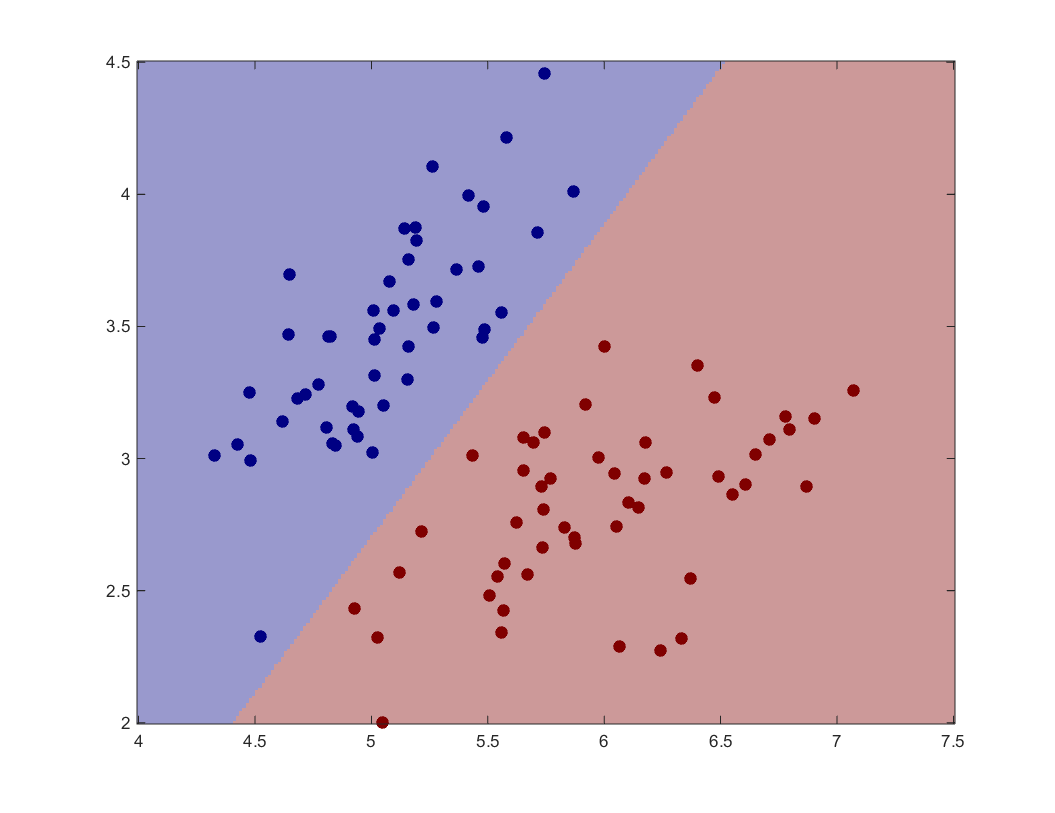
\includegraphics[width=6 in]{prob1Plot1.png}
\caption{Classification Plot with support vectors starred in yellow}
\end{figure}
\newpage
Here is the code to obtain the previous plot. The details of how I transformed into a version compatible with quadprog are in the comments. 
\lstinputlisting[firstline=1, lastline=49]{prob1.m}

\newpage

This is the code to obtain $\alpha$, verify it, and then plot the classification bounday. 
\lstinputlisting[firstline=51, lastline=119]{prob1.m}

\newpage

\section*{Problem 2}

\subsection*{Part a}

To calculate the entropy, I did the following
\[
H(y) = p(y=1)log_2(\frac{1}{p(y=1)}) + p(y=-1)log_2(\frac{1}{p(y=-1)})
\]
The entropy ends up being $0.9743$
\\

\subsection*{Part b}

You should split on feature 2 first. Here is the information gain for all the variables:\\
\\
\begin{tabular}{ c | c }
  Feature & Information Gain\\
  \hline                       
  1 & 0.0245 \\
  2 & 0.5059 \\
  3 & -0.0097 \\
  4 & 0.0930 \\
  5 & -0.0095 \\      
\end{tabular}

\newpage

\subsection*{Code for a and b}

This is the code to complete Part A and B. The code for the getEntropy function will be shown later.

\lstinputlisting[firstline=1, lastline=48]{prob2.m}

\subsection*{Part C}

Here is the decision tree for Part C

\begin{figure}[h]
\centering

\includegraphics[width=6 in]{hw4prob2DecisionTree.png}
\caption{Decision Tree}
\end{figure}

\newpage

Here is the code used in Part C. It relies on the data set up from Part A.

\lstinputlisting[firstline=50, lastline=82]{prob2.m}

\subsection*{Matlab functions written for Problem 2}

This is the code for the getEntropy function
\lstinputlisting[firstline=1, lastline=15]{getEntropy.m}

This is the code for the getDecTreeSplit function
\lstinputlisting[firstline=1, lastline=52]{getDecTreeSplit.m}


\section*{Problem 3}

\subsection*{Part a}

The validation MSE that I obtained was 0.7133. \\
This is the code I used to obtain it:
\lstinputlisting[firstline=1, lastline=11]{prob3.m}

\newpage

\subsection*{Part b}

At the maxDepth parameter increases, the model grows increasingly complex. This is due to the fact that more nodes can be added to the decision tree. Just like with other models, it does begin to overfit as we add complexity. The lowest validation MSE is obtained when maxDepth is 8 and after that overfitting seems to begin. The validation MSE at 8 ends up being 0.4355. Here is the plot which illustrates that below.

\begin{figure}[h]
\centering
\includegraphics[width=6 in]{prob3plot1.png}
\caption{Validation MSEs for the Decision Trees with varying maxDepth}
\end{figure}

\newpage

Here is the code used for Part b\\
\lstinputlisting[firstline=13, lastline=29]{prob3.m}

\newpage

\subsection*{Part c}

With the minParent parameter, the model grows decreasingly complex as minParent grows. This is due to the fact that the number of data points required for a new split increases, hence less splits will be made. Thus it goes from overfitting to underfitting as minParent grows. It is thus overfitting in the first few steps and underfitting in the last few steps. The best validation MSE is obtained in the middle when minParent is equal to $2^9$ with an MSE of 0.4306. Here is the plot which illustrates this:

\begin{figure}[h]
\centering
\includegraphics[width=6 in]{prob3plot2.png}
\caption{Validation MSEs for the Decision Trees with varying minParent}
\end{figure}

\newpage

Here is the code used for Part c\\
\lstinputlisting[firstline=31, lastline=46]{prob3.m}

\newpage

\subsection*{Part d}

I attempted 3 different calls to treeRegress with the following parameters:\\
1. maxDepth=9, minParent=$2^9$\\
2. maxDepth=20, minParent=$2^9$\\
3. maxDepth=9\\
\\
With call 1, the Kaggle score was 0.65140\\
With call 2, the Kaggle score was 0.64843, which was the best one of the three\\
With call 3, the Kaggle score was 0.66217\\

Here is the code for part d\\
\lstinputlisting[firstline=48, lastline=68]{prob3.m}

\newpage

\section*{Problem 4}

\subsection*{Part a}

I decided to do Option 2 and employ Gradient Boosting to try to enhance my predictions. \\
Here are the errors I got for 1,5,10,25 learners: \\
\\
\begin{tabular}{ c | c | c }
  Number of Learners & Training MSE & Validation MSE\\
  \hline                       
  1 & 0.6203 & 0.6461 \\
  5 & 0.4933 & 0.4386\\
  10 & 0.4487 & 0.4136\\
  25 & 0.4283 & 0.3923\\
\end{tabular}
\\
\\
Here is the plot of training and validation MSE:\\
\begin{figure}[h]
\centering
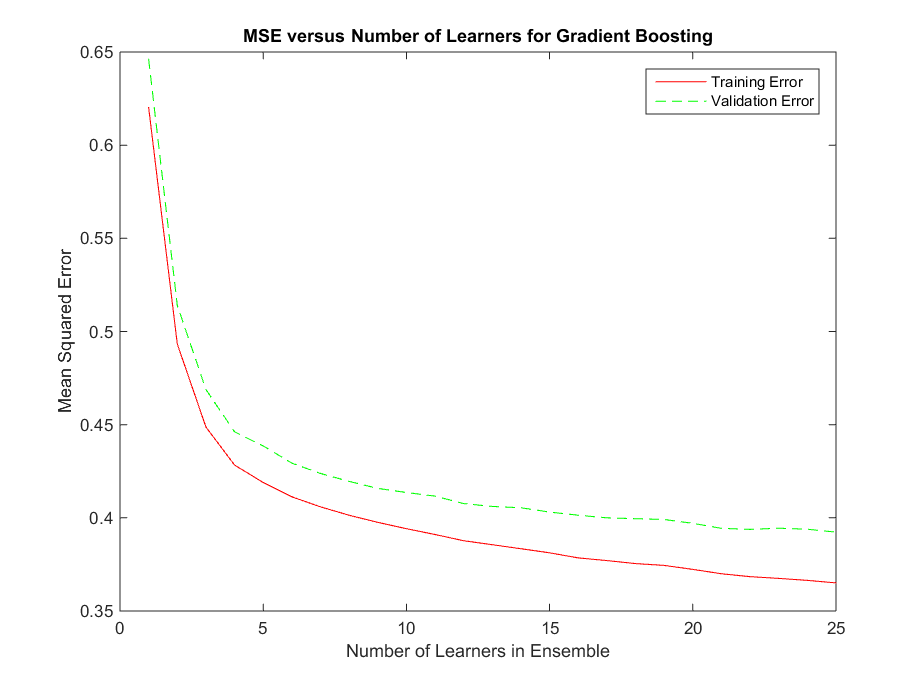
\includegraphics[width=6 in]{prob4PartA.png}
\caption{MSE versus number of learners}
\end{figure}

\newpage

Here is the code for Part A, which uploaded the data, trained the ensembles, and then graphed the results.
\lstinputlisting[firstline=1, lastline=51]{prob4.m}

\newpage

\subsection*{Part b}

After having over 200 learners trained and seeing the validation error, the lowest validation error was reached at 0.3787 when there were 82 learners. I have decided to retrain on all the test data and have it learn 100 learners before running it on the test data. \\
\\
After uploading to Kaggle, my score was $0.61760$.\\
\\
Here is the code for Part B, which trained the ensembles on all the training data and then made the Kaggle file. It uses some of the variables in Part A that were created to hold the data. \\
\lstinputlisting[firstline=52, lastline=78]{prob4.m}


\end{document}
